% Chapter Template

\chapter{Попередня обробка даних} % Main chapter title

\label{Chapter2} % Change X to a consecutive number; for referencing this chapter elsewhere, use \ref{ChapterX}

%----------------------------------------------------------------------------------------
%	SECTION 1
%----------------------------------------------------------------------------------------

\section{Сегментація ядер}

\begin{figure}[b!]
	\minipage{0.333\textwidth}
	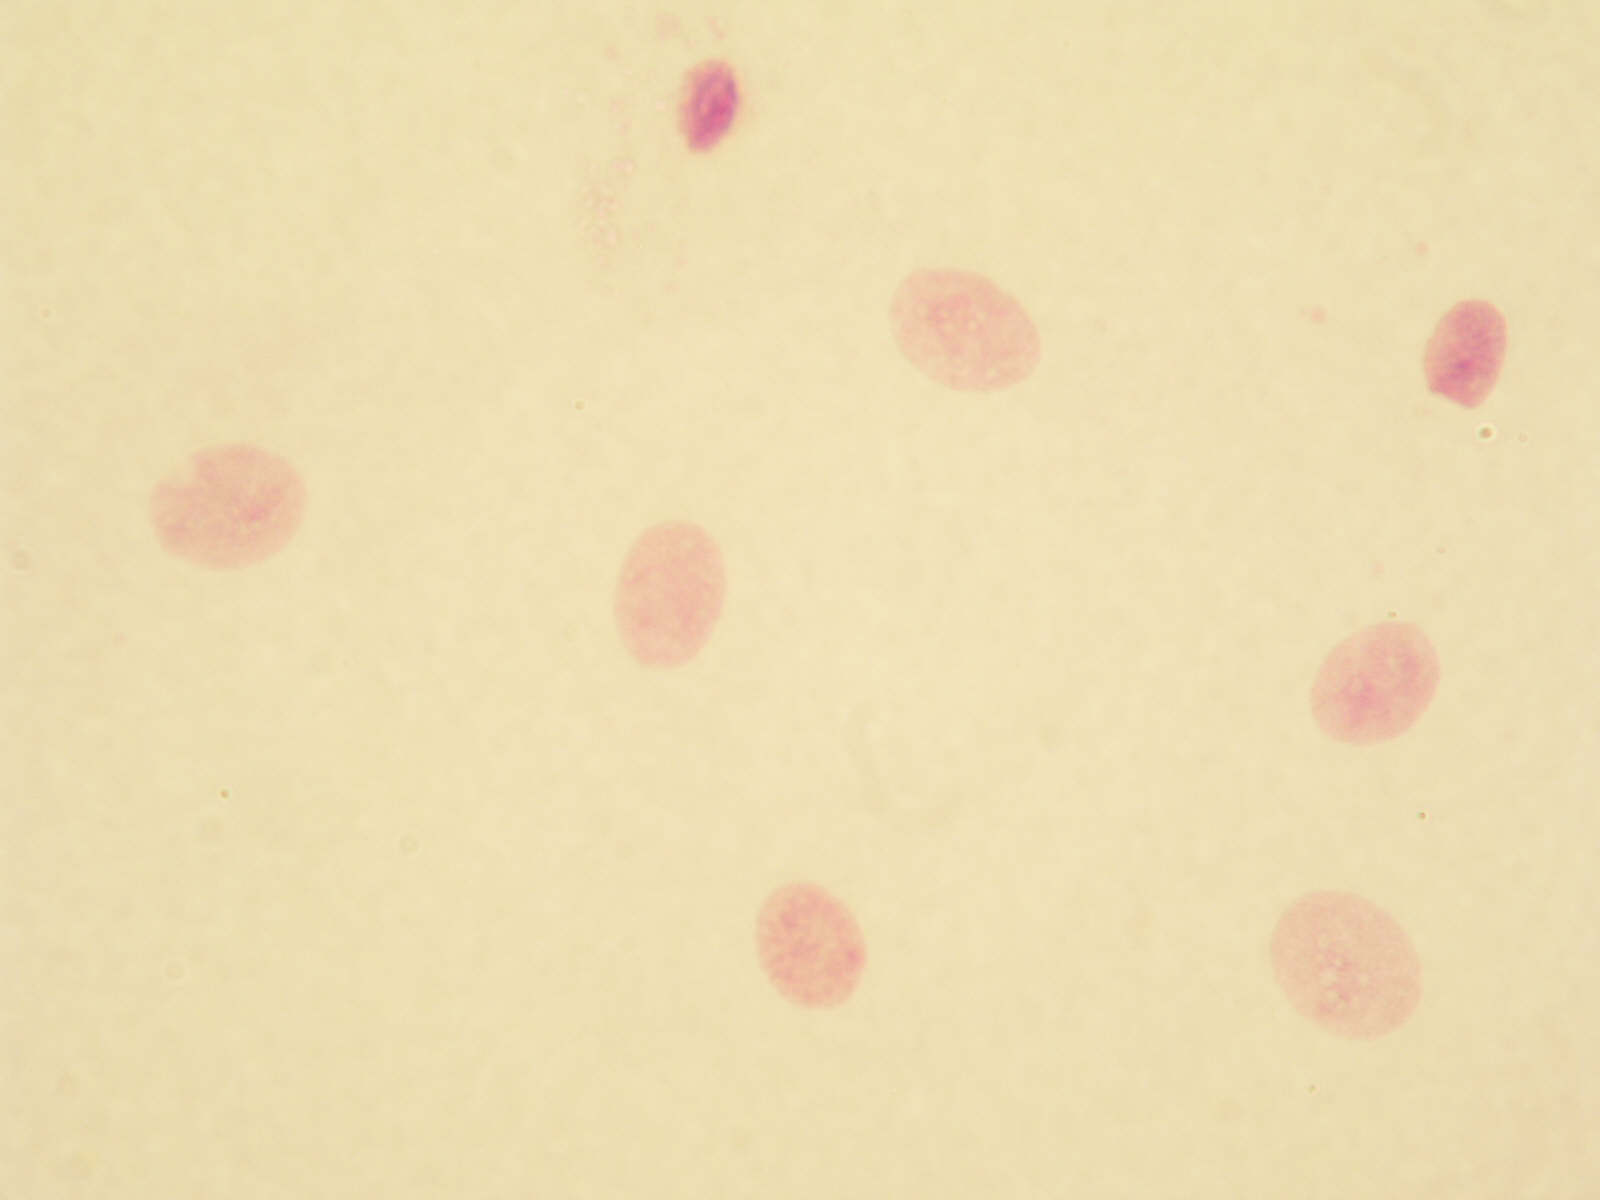
\includegraphics[width=0.97\linewidth]{Figures/Chapter2/0a.png}
	\centering
	\endminipage\hfill
	\minipage{0.333\textwidth}
	\centering	
	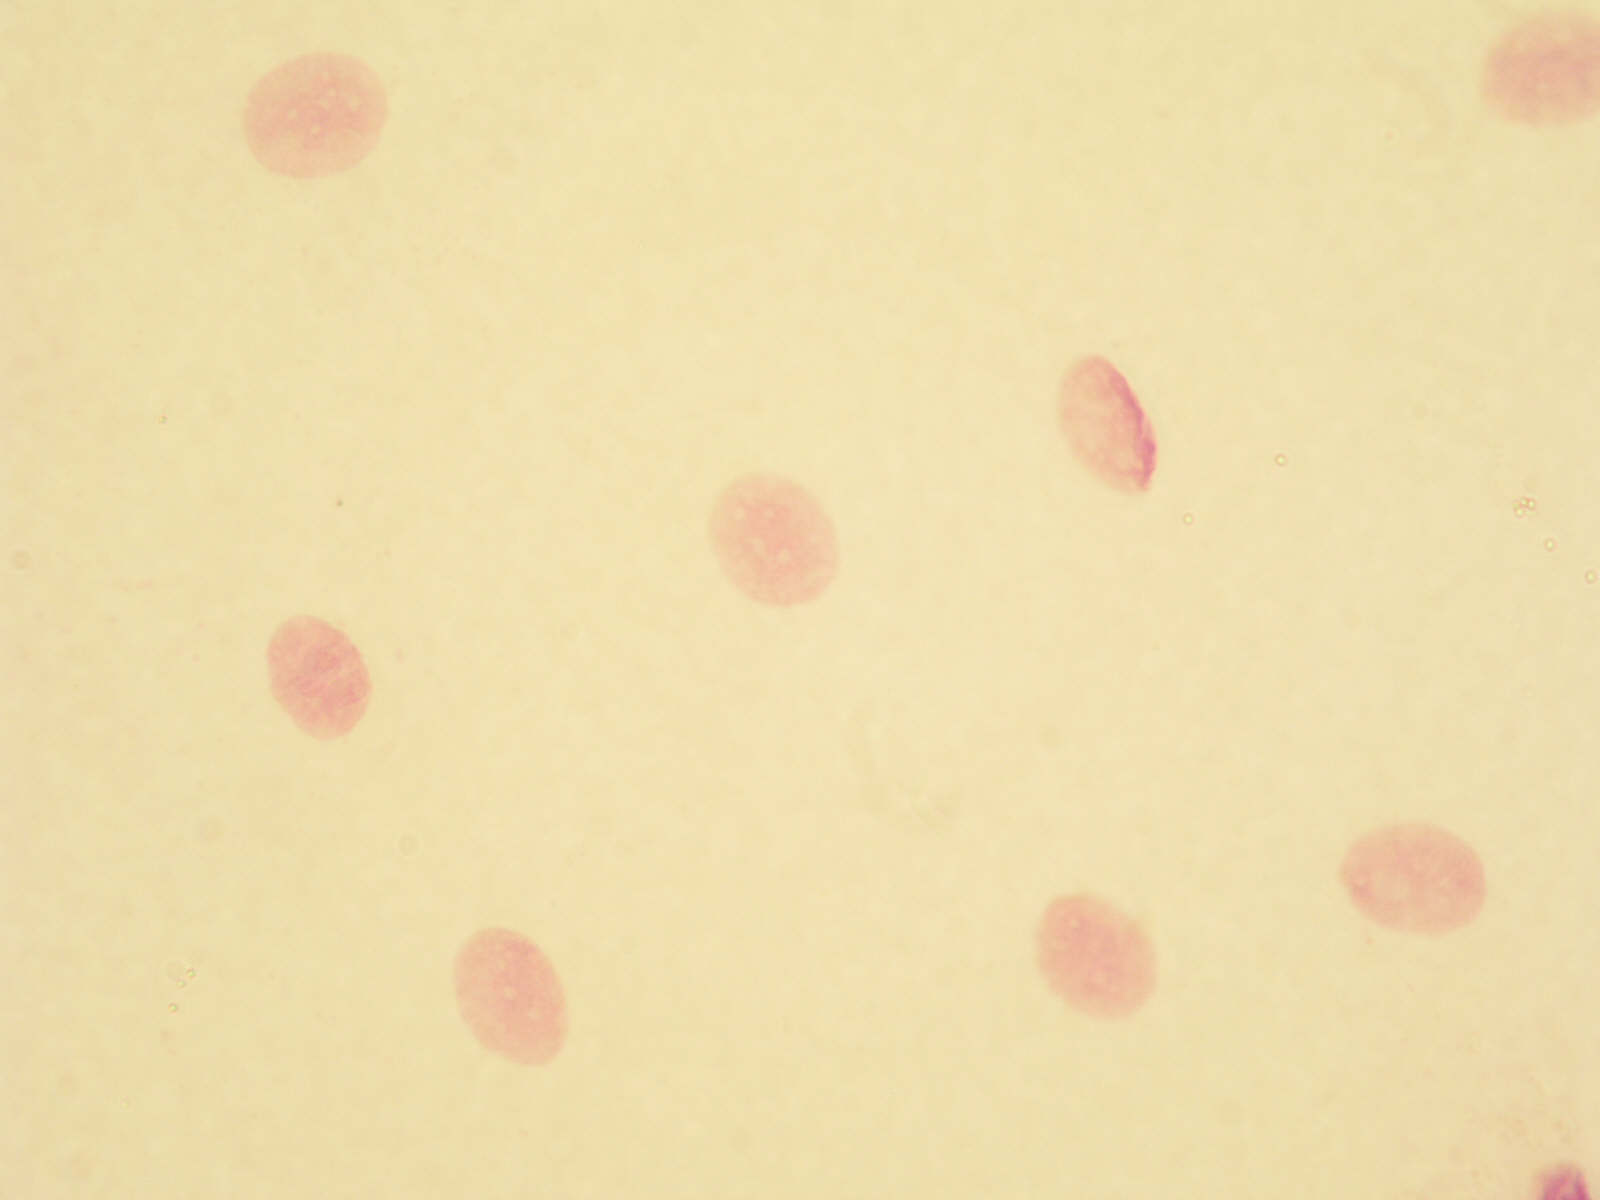
\includegraphics[width=0.97\linewidth]{Figures/Chapter2/0b.png}
	\endminipage\hfill
	\minipage{0.333\textwidth}
	\centering	
	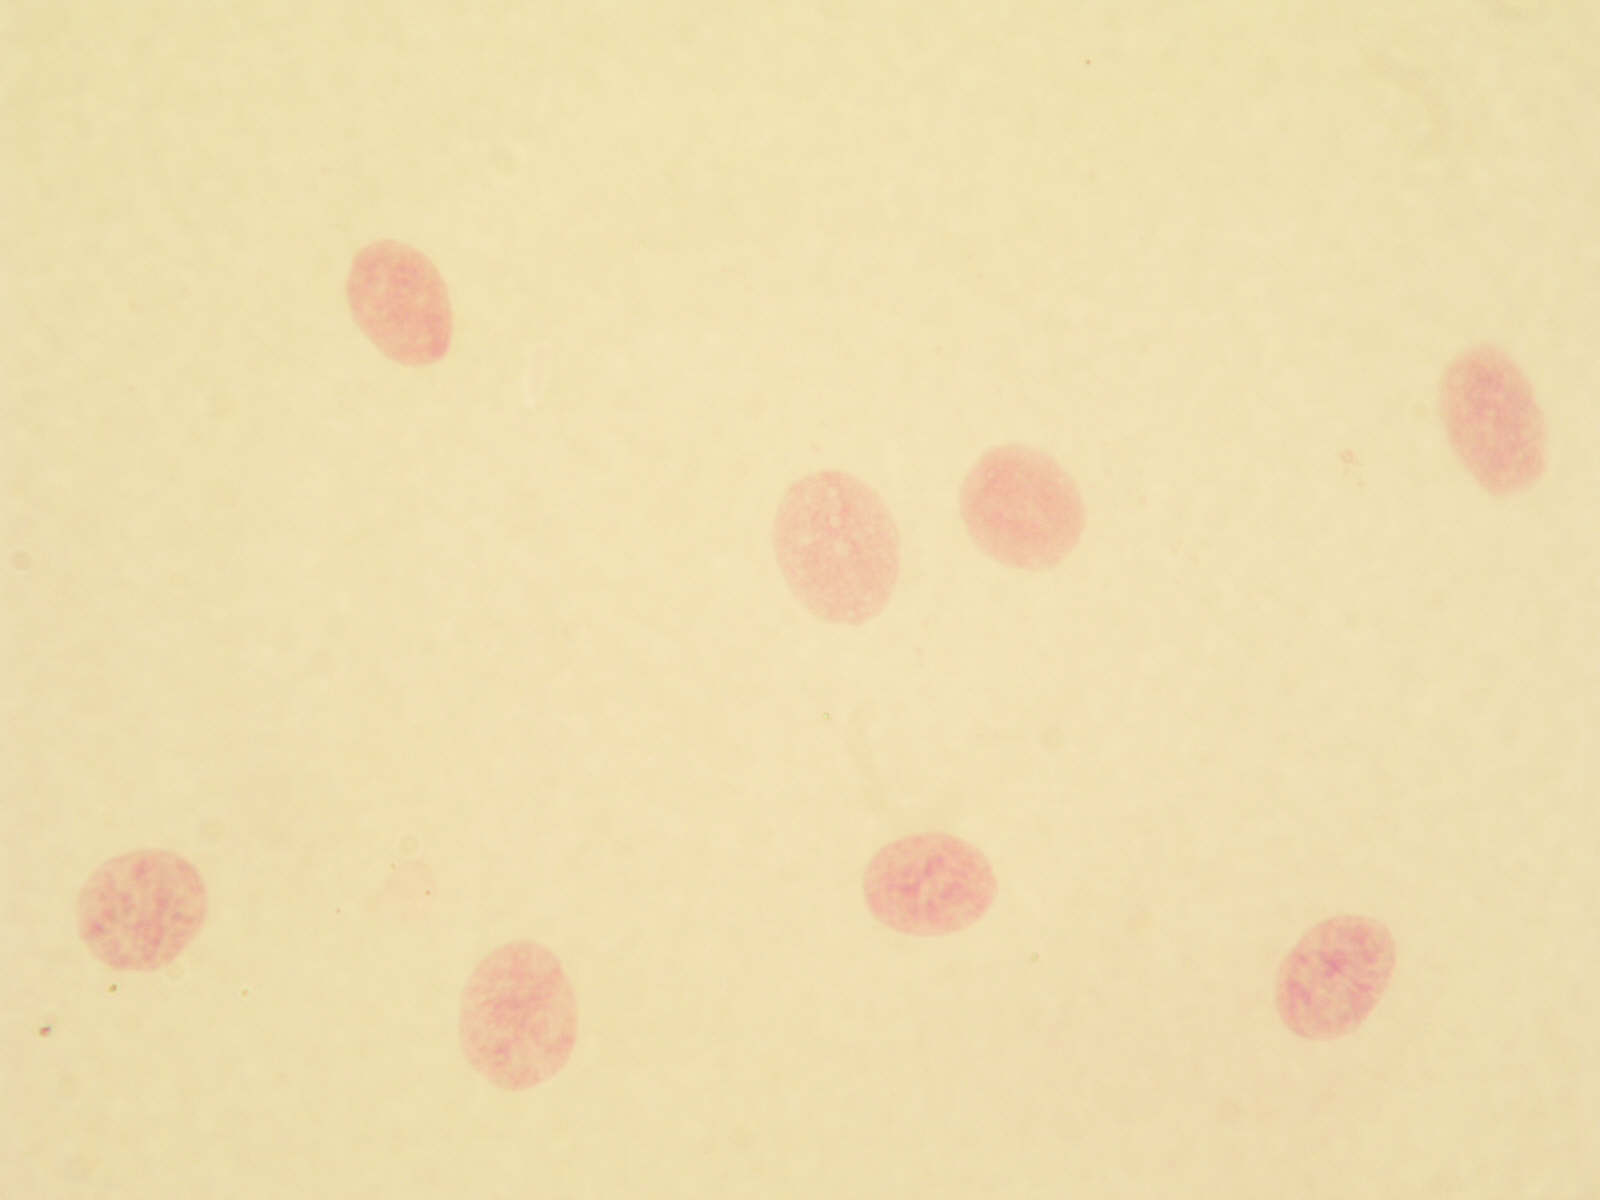
\includegraphics[width=0.97\linewidth]{Figures/Chapter2/0c.png}
	\endminipage\hfill
	
	\caption{Зображення інтерфазних ядер букального епітелію, які треба сегментувати.}
	\label{fig:raw_cells}
\end{figure}

\par
Мікроскопічні зображення у чистому вигляді зазвичай неприйнятні для аналізу у зв’язку з наявністю дефектів, цифрових шумів, спричинених необхідністю підвищення світло- чутливості фотоматеріалів, а також сторонніх об’єктів. Отже, для подальшого аналізу вхідного набору зображень (або набору пацієнтів), необхідно зробити попередню обробку та сегментацію.

\par
На (Мал.~\ref{fig:raw_cells}) зображено приклади знімків інтерфазних ядер букального епітелію. З них треба виділити окремі клітини для подальшого аналізу. Задача обробки та сегментації зображень розбивається на наступні підзадачі:

\begin{enumerate}
	\item Зменшення шуму
	\item Відділення фону
	\item Виділення окремого ядра клітини
\end{enumerate}

\par
Перша та друга підзадачі стандартно розв’язуються за допомогою алгоритмів фільтрації зображень, а друга підзадача розв’язується за допомогою алгоритму бінаризації Оцу. 

У загальному випадку, якщо на зображенні присутні різні об'єкти (у даному випадку -- ядра різних типів клітин чи різні клітини), третя підзадача дуже складно розв’язується детермінованими алгоритмами, оскільки об'єкти можуть перекриватися, торкатися один одного та мати абсолютно різні форми, кольори та розміри. Так, наприклад, \citep{bib:cellcount} вико- ристав нейронні мережі для класифікації та сегментації зображень клітин.

У нашому випадку, на досліджуваних зображеннях присутні тільки інтерфазні ядра букального епітелію. Отже, ми припускаємо, що радіуси цих ядер приблизно однакові та можемо використовувати алгоритми на основі морфологічних операцій, трансформації відстані та алгоритму водоподілу, які будуть детально розглянуті далі.

\subsection{Зменшення шуму. Медіанна фільтрація.}

Для зменшення рівня шуму знімків мікроскопа будемо використовувати медіанний фільтр -- один з видів цифрових фільтрів, запропонований \citep{bib:medianfilter}, що широко застосовується в цифровій обробці сигналів та зображень. Його використання дає найкращі результати для збереження перепадів відтінків, різноманітних кордонів та локальних піків яскравос- ті на спотворених імпульсним шумом зображеннях. Швидкий алгоритм медіанної філь- 	трації виглядає наступним чином:


\begin{megaalgorithm}[H]
	\label{alg:medianfilter}
	\caption{Медіанна фільтрація}
	\SetKwInOut{Input}{Вхід}\SetKwInOut{Output}{Вихід}
	
	\Input{Зображення $X$ розміром $m \times n$, радіус ядра (вікна фільтру) $r$}
	\Output{Зображення $Y$ такого ж розміру}
	\BlankLine 
	
	Ініціалізація гістограму ядра $H$\;
	
	\For{$i = 1 \textup{ to } m $}{
		\For{$j = 1 \textup{ to } n $}{
			\For {$k = -r \textup{ to } r $}{
				Вилучити $X_{i+k,j-r-1}$ від $H$\;
				Додати $X_{i+k,j+r}$ до $H$\;
			}
			$Y_{i,j} \leftarrow \textup{медіана} (H)$\;
		}
	}
\end{megaalgorithm}

\begin{figure}[t!]
	\minipage{0.2\textwidth}
	\centering
	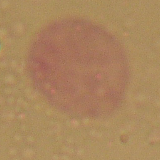
\includegraphics[width=0.95\linewidth]{Figures/Chapter2/1a.png}
	Оригінал
	\endminipage\hfill
	\minipage{0.2\textwidth}
	\centering	
	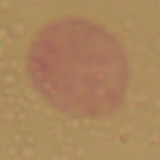
\includegraphics[width=0.95\linewidth]{Figures/Chapter2/1b.png}
	При \(k = 3\)
	\endminipage\hfill
	\minipage{0.2\textwidth}
	\centering	
	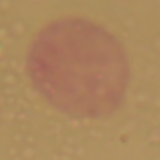
\includegraphics[width=0.95\linewidth]{Figures/Chapter2/1c.png}
	При \(k = 5\)
	\endminipage\hfill
	\minipage{0.2\textwidth}
	\centering	
	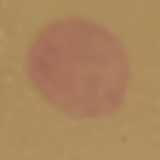
\includegraphics[width=0.95\linewidth]{Figures/Chapter2/1d.png}
	При \(k = 9\)
	\endminipage\hfill
	\minipage{0.2\textwidth}
	\centering	
	
\includegraphics[width=0.95\linewidth]{Figures/Chapter2/1e.png}
	При \(k = 13\)
	\endminipage\hfill	
	
	\caption{Дія медіанного фільтру на зображення.}
	\label{fig:median_cells}
\end{figure}

На (Мал. \ref{fig:median_cells}) показано, як змінюється рівень шуму та чіткість зображення в залежності від розміру вікна фільтру \(k = 2r + 1\). Можна побачити, що при \(k = 3\), зображення мінімально позбавлене шуму, а текстура ядра майже повністю зберігається. При \(k = 13\) дуже гарно виділяються контури ядра клітини та зображення зовсім позбавлене шуму, але майже повністю втрачено текстуру ядра.

Отже, на різних етапах аналізу можна використовувати медіанні фільтри з різними розмірами вікна фільтру. Наприклад, при сегментації зображень (Мал. \ref{fig:raw_cells}) доречно використовувати вікна фільтру з великими розмірами, оскільки на цьому етапі нас більше цікавлять контури об'єктів, а при класифікації (здоровий, хворий раком або фіброаденоматозом) краще використовувати якомога менші вікна фільтру, оскільки нас цікавить текстура інтерфазного ядра клітини букального епітелію.


\subsection{Відділення фону. Бінаризація Оцу.}

\par
Наступний етап обробки зображення -- відділення фонових пікселів від пікселів об'єктів, наявних на зображенні (ядер клітин або сторонніх об'єктів). Для досягнення цієї мети підходить алгоритм бінаризації зображення Оцу \parencite{bib:otsu}. 

\par

Нехай пікселі зображення приймають значення у $L$ рівнях сірого кольору, тобто значення з множини $\left\{ 1, 2, \dots, L \right\}$, кількість пікселів зі значенням $i$ дорівнює $n_i$, а кількість пікселів у зображенні -- $N$. Треба розділити множину пікселів на два класи $C_0$ та $C_1$ (фонові пікселі та пікселі об'єктів, або навпаки) за допомогою деякого значення порогу $k$. До $C_0$ віднесемо усі пікселі зі значеннями з $\left\{ 1, 2, \dots, k \right\}$, а до $C_1$ -- усі пікселі зі значеннями з множини $\left\{ k+1, k+2, \dots, L \right\}$. Нехай $\omega_0$ та $\omega_1$ -- частота класів $C_0$ та $C_1$ відповідно.  

$$\omega_0 = \omega_0(k) = \sum_{i=0}^{k}{\frac{n_i}{N}}, \quad
\omega_1 = \omega_1(k) = \sum_{i=k+1}^{k}{\frac{n_i}{N}} = 1 - \omega_0$$

оді метод Оцу полягає у пошуку порогу $k$, який мінімізує дисперсію в середині класу, яка визначається як зважена сума дисперсій двох класів:

$$\sigma_{\omega}^{2}(k) = \sigma_{0}^2(k) \omega_0(k) + \sigma_{1}^2(k) \omega_1(k) \rightarrow \min$$

Де $\sigma_{0}^2(k)$ та $\sigma_{2}^2(k)$ -- дисперсія класів $C_0$ та $C_1$ для порогу $k$ відповідно. У своїй роботі Оцу також показав, що мінімізація дисперсії в середині класу рівносильна максимізації дисперсії між класами:

$$\sigma_{b}^2(k) = \omega_0(k)\omega_1(k) \left( \mu_0(k) - \mu_1(k) \right)^2 \rightarrow \max$$

Де $\mu_0(k)$ та $\mu_1(k)$ -- середнє арифметичне класів $C_0$ та $C_1$ при порозі $k$ відповідно, тобто:

$$\mu_T = {{\sum^{L}_{i=0} {i \cdot n_i}} \over {N}} $$
$$\mu_0(k) = {{\sum^{t-1}_{i=0} {i \cdot n_i}} \over {N \cdot \omega_0(k)}}, \quad \mu_1(t) = {{\mu_T - \mu_0(k) \cdot \omega_0(k)} \over {\omega_1(k)}}.$$

Значення $\omega_0(k+1)$, $\omega_1(k+1)$, $\mu_0(k+1)$ та $\mu_1(k+1)$ достатньо легко виражаються через значення $\omega_0(k)$, $\omega_1(k)$, $\mu_0(k)$ та $\mu_1(k)$, що дозволяє швидко обчислити оптимальний поріг $k$. Отже, алгоритм бінаризації Оцу виглядає наступним чином:

\begin{megaalgorithm}[H]
	\caption{Бінаризація зображення Оцу}
	\SetKwInOut{Input}{Вхід}\SetKwInOut{Output}{Вихід}
	
	\Input{Зображення $X$ розміром $m \times n$}
	\Output{Поріг $k$}
	\BlankLine 
	
	\textbf{обчислити} гістограму $n_i$ зображення та частоту $N(i) = \frac{n_i}{N}$ для кожного рівня інтенсивності зображення $X$\;
	\textbf{обчислити} початкові значення $\omega_0(0)$, $\omega_1(0)$, $\mu_0(0)$ та $\mu_1(0)$\;
	\textbf{поставити} $\sigma_{\max}^2 \leftarrow 0$\;
	\For{$k = 1 \textup{ to } L $}{
		\textbf{Оновити} значення $\omega_0(k)$, $\omega_1(k)$, $\mu_0(k)$ та $\mu_1(k)$\;
		\textbf{Обчислити} $\sigma_{b}^2(k) = \omega_0(k)\omega_1(k) \left( \mu_0(k) - \mu_1(k) \right)^2$\;		
		\If{$\sigma_{b}^2(k) > \sigma_{\max}^2$}{
			\textbf{поставити} $\sigma_{\max}^2 \leftarrow \sigma_{b}^2(k)$
		}
	}
	\textbf{поставити} $k \leftarrow \sigma_{\max}^2$\;
\end{megaalgorithm}

\begin{figure}[t!]
	\minipage{0.5\textwidth}
	\centering
	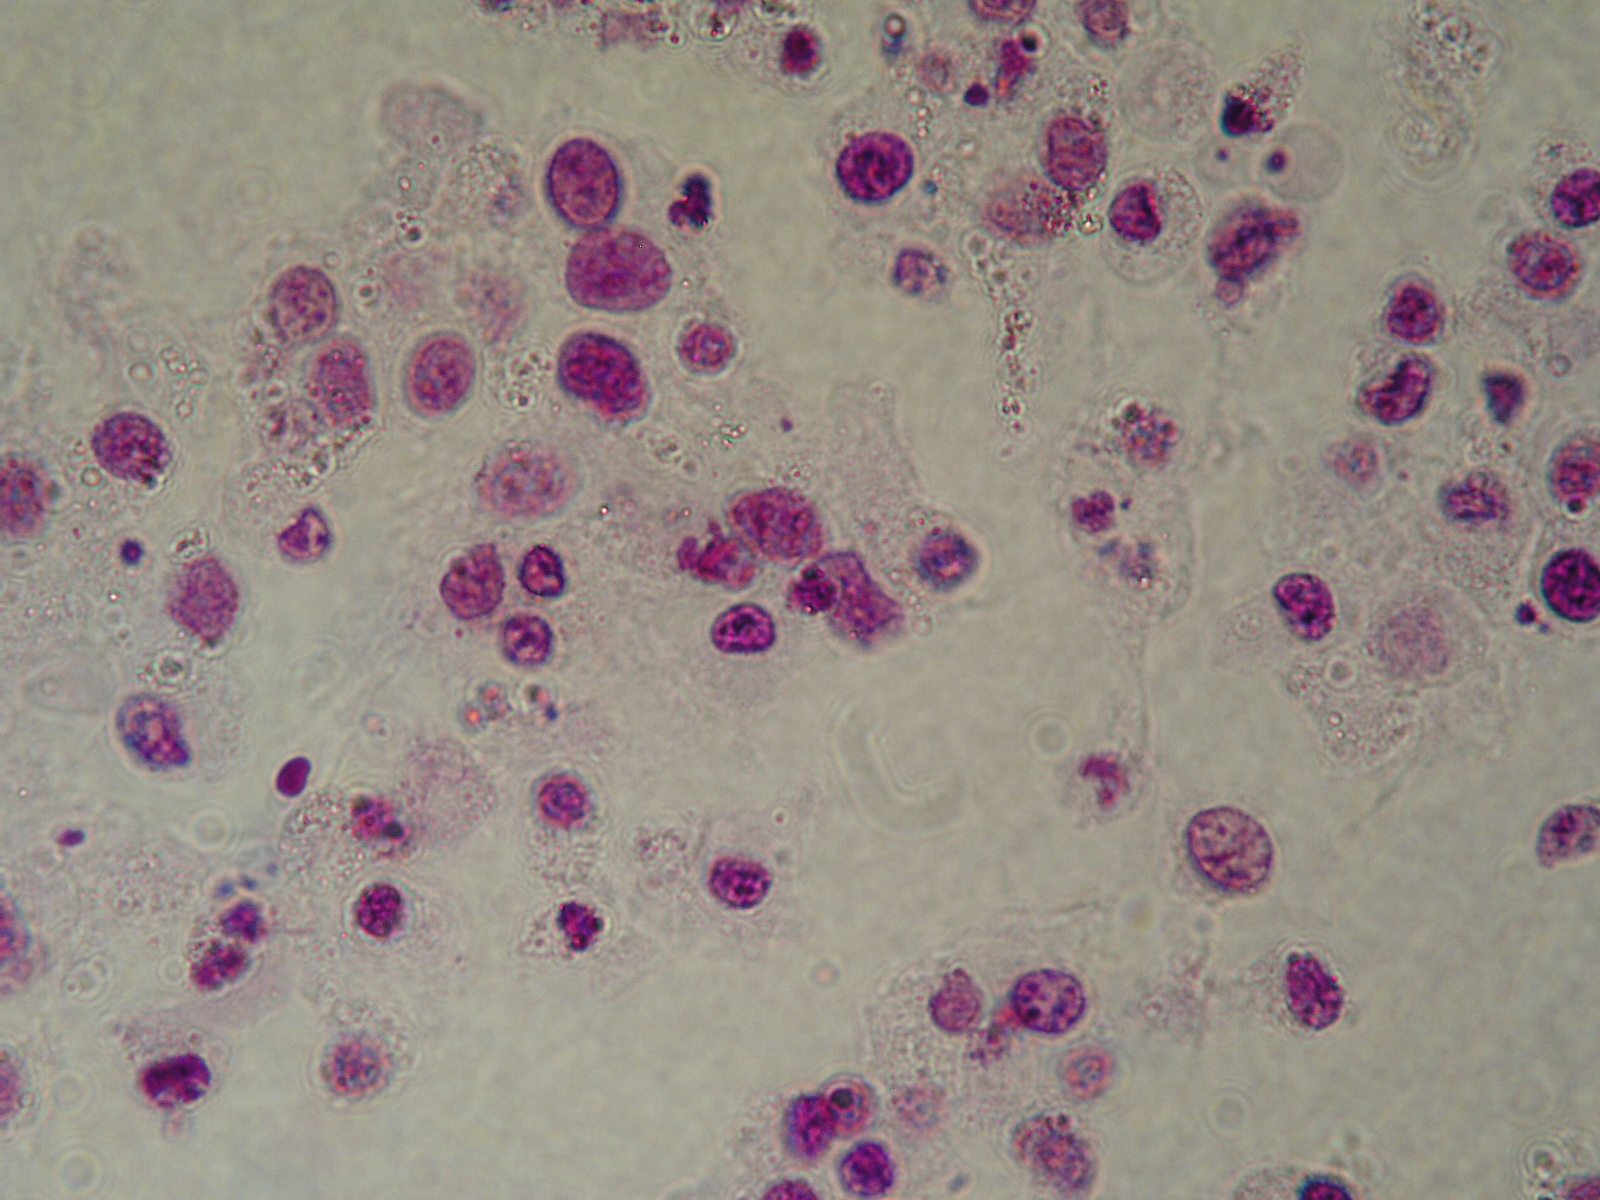
\includegraphics[width=0.97\linewidth]{Figures/Chapter2/2a.png}
	\endminipage\hfill
	\minipage{0.5\textwidth}
	\centering	
	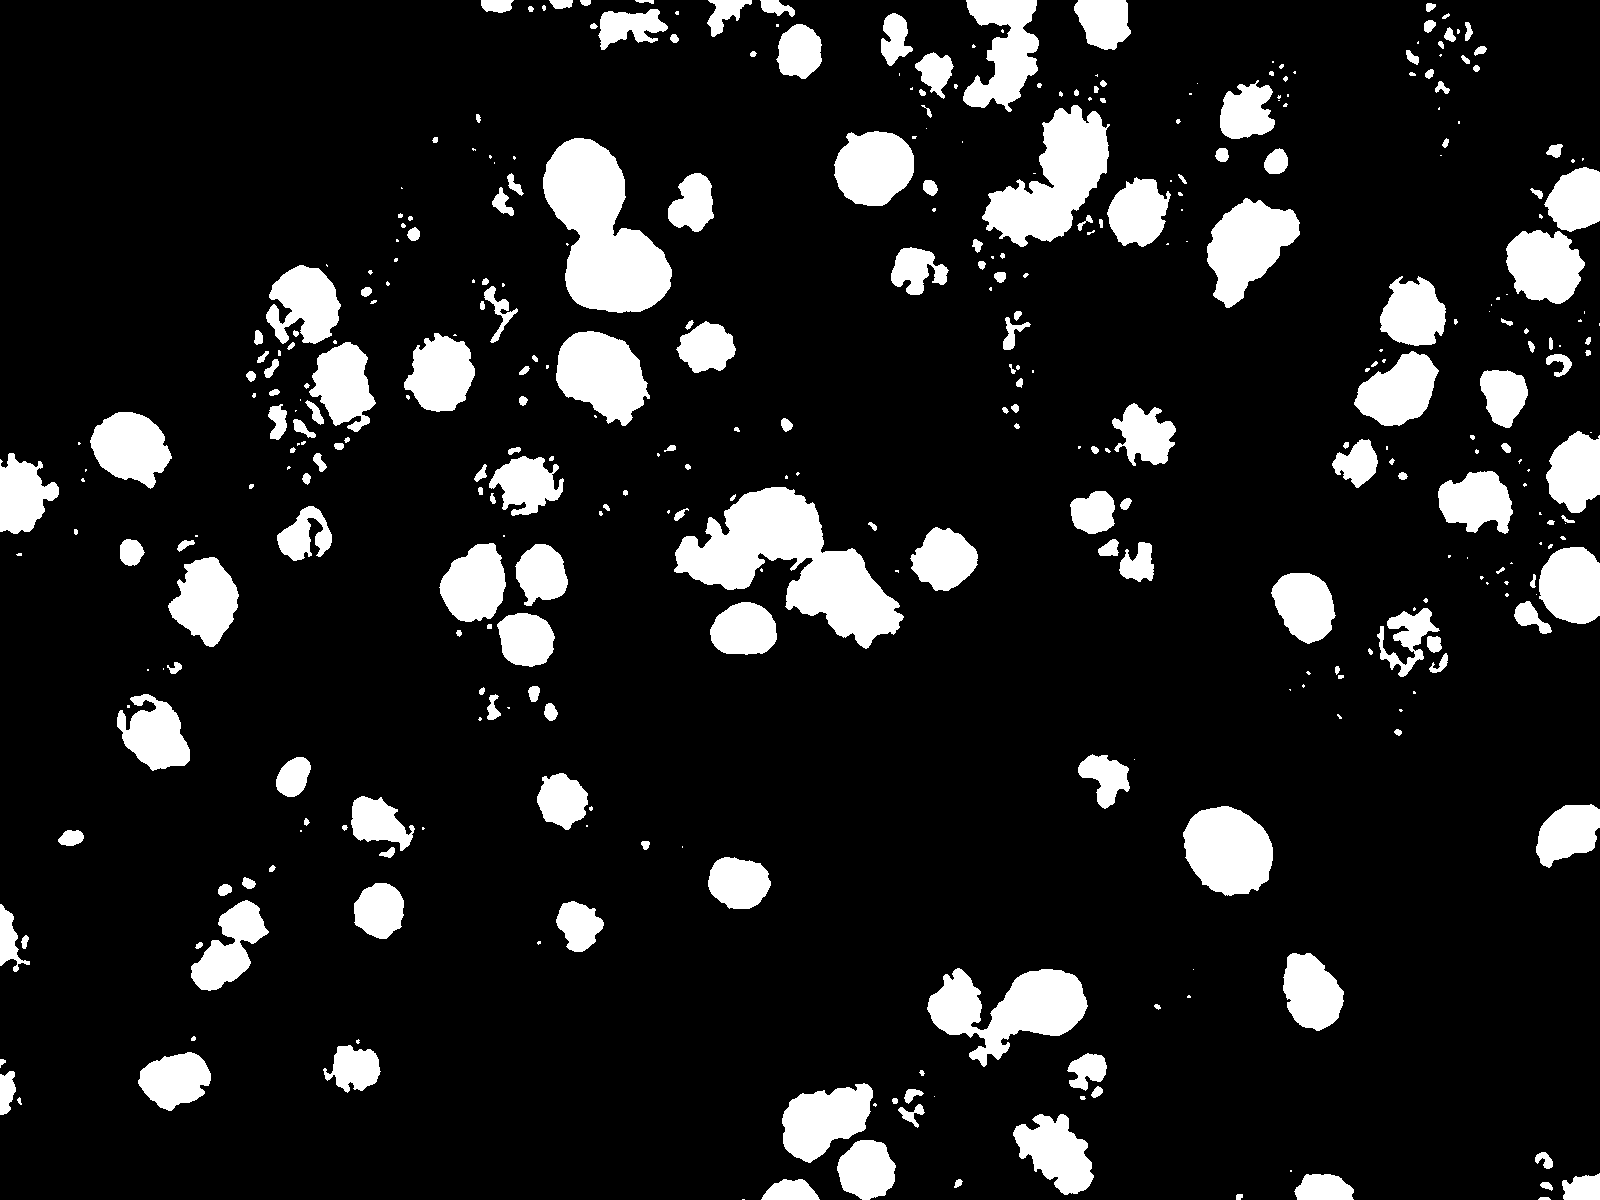
\includegraphics[width=0.97\linewidth]{Figures/Chapter2/2b.png}
	\endminipage\hfill	
	
	\caption{Результат бінаризації.}
	\label{fig:binarized_cells}
\end{figure}

\par
На зображенні (Мал. \ref{fig:binarized_cells}) результат бінаризації фільтрованого медіанним фільтром зобра- ження з розміром \(k = 5\). Негладкі контури інтерфазних ядер клітин після бінаризації, а також неточності у деяких регіонах зображення нас не турбують на даному етапі, оскільки це можна виправити морфологічними операціями, які будуть детально розгля- нуті далі.


\subsection{Бінарні морфологічні операції над зображеням.}

У бінарній морфології, зображення розглядається як підмножина Евклідового простору \(\mathbb{R}^d\) або цілочисельної сітки \(\mathbb{Z}^d\), де \(d\) -- розмірність простору. Операції морфології застосо- вуються до зображень разом з заданим структурним елементом, або ядром, яке визначає природу операції. Для обробки зображень найчастіше використовують наступний струк- турний елемент:
\begin{equation*}
B = \{ (-1, -1), (-1, 0), (-1, 1), (0, -1), (0, 0), (0, 1), (1, -1), (1, 0), (1, 1)\}\,.
\end{equation*}

Двома основними морфологічними операціями є Erosіon(звуження) і Dіlatіon(розширення). Операція звуження зображення задається наступним чином:
\begin{equation*}
A \ominus B = \left\{ z \in \mathbb{Z}^d | B_z \subseteq A \right\}\,,
\end{equation*}
де \(A\) -- зображення, \(B\) -- структурний елемент, \(B_z\) -- трансляція вектору \(z\), тобто
\begin{equation*}
B_z = \left\{ b + z | b \in B \right\}, \quad \forall z \in \mathbb{Z}^d
\end{equation*}

Ідея цієї операції полягає в наступному. Ядро (структурний елемент) ковзає по зобра- женню. Піксель в бінаризованому зображенні (1 або 0) буде вважатися 1, тільки якщо всі пікселі під ядром рівні 1, в іншому випадку він буде зруйнований (стане рівним нулю). Таким чином, в результаті операції всі пікселі, що знаходяться на краю, будуть відкинуті в залежності від розміру ядра. Таким чином, товщина або розмір об'єкта переднього плану зменшується. Цей метод може використовуватися для видалення невеликих шумів, роз’єднання двох пов'язаних об'єктів та іншого.

Операція розширення зображення задається наступним чином:
\begin{equation*}
A  \oplus B = \bigcup_{b\in B} A_b\,.
\end{equation*}

Ця операція протилежна ерозії. Тут піксель бінаризованого зображення  дорівнює \enquote{1}, якщо принаймні один піксель під ядром дорівнює \enquote{1}. Таким чином, збільшується біла область зображення або збільшується розмір об'єкта переднього плану. Зазвичай у ви- падках, коли потрібно видалити шум навколо об’єкта, спочатку використовують опера- цію звуження, а потім операцію розширення. Розширення необхідне, оскільки ерозія, крім видалення білого шуму, скорочує наш об'єкт. 

\begin{figure}[t!]
	\minipage{0.333\textwidth}
	\centering
	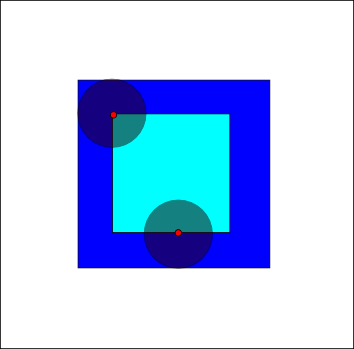
\includegraphics[width=0.80\linewidth]{Figures/Chapter2/Erosion.png}
	Звуження \(\ominus\)
	\endminipage\hfill
	\minipage{0.333\textwidth}
	\centering	
	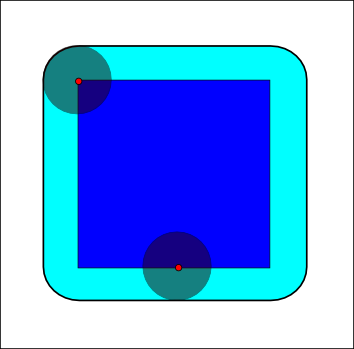
\includegraphics[width=0.80\linewidth]{Figures/Chapter2/Dilation.png}
	Розширення \(\oplus\)
	\endminipage\hfill
	\minipage{0.333\textwidth}
	\centering	
	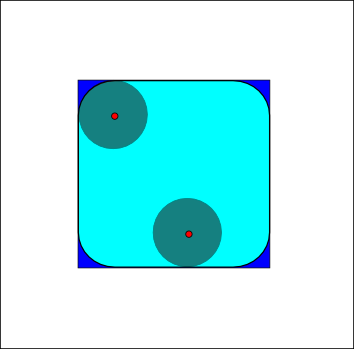
\includegraphics[width=0.80\linewidth]{Figures/Chapter2/Opening.png}
	Відкриття \(\circ\)
	\endminipage\hfill
	
	\caption{Морфологічні операції з круглим структурним елементом над синім квадратом.}
	\label{fig:morphology_explained}
\end{figure}

На основі основних операцій звуження (\(\ominus\)) та розширення (\(\oplus\)) задаються інші операції. Операція морфологічного відкриття (openіng) задається наступним чином:
\begin{equation*}
A \circ B  = (A \ominus B) \oplus B\,.
\end{equation*}

або
\begin{equation*}
A \circ Bс = \mathop\bigcup\limits_{B_{{\textbf{z}}}\subseteq A} {B_{{\textbf{z}}}}.
\end{equation*}

У \citep{book:serra} більш детально розглянуто теоретичні та практичні аспекти операції математичної морфології.

Позначимо зображення, отримане у результаті розширення бінарного зображення за 2 ітерації у (\ref{fig:morph_cells}) як \(zoneOfinterest\). Очевидно, що всі пікселі, які дорівнюють \(0\) у \(sureBG\) є пікселями фону. Отже, ядра треба шукати тільки серед тих точок \(zoneOfinterest\), які дорівнюють \(1\) (позначено білим кольором). Позначимо також відкриття у (Мал. \ref{fig:morph_cells}) як \(threshOpenіng\).

\begin{figure}[b!]
	\minipage{0.5\textwidth}
	\centering	
	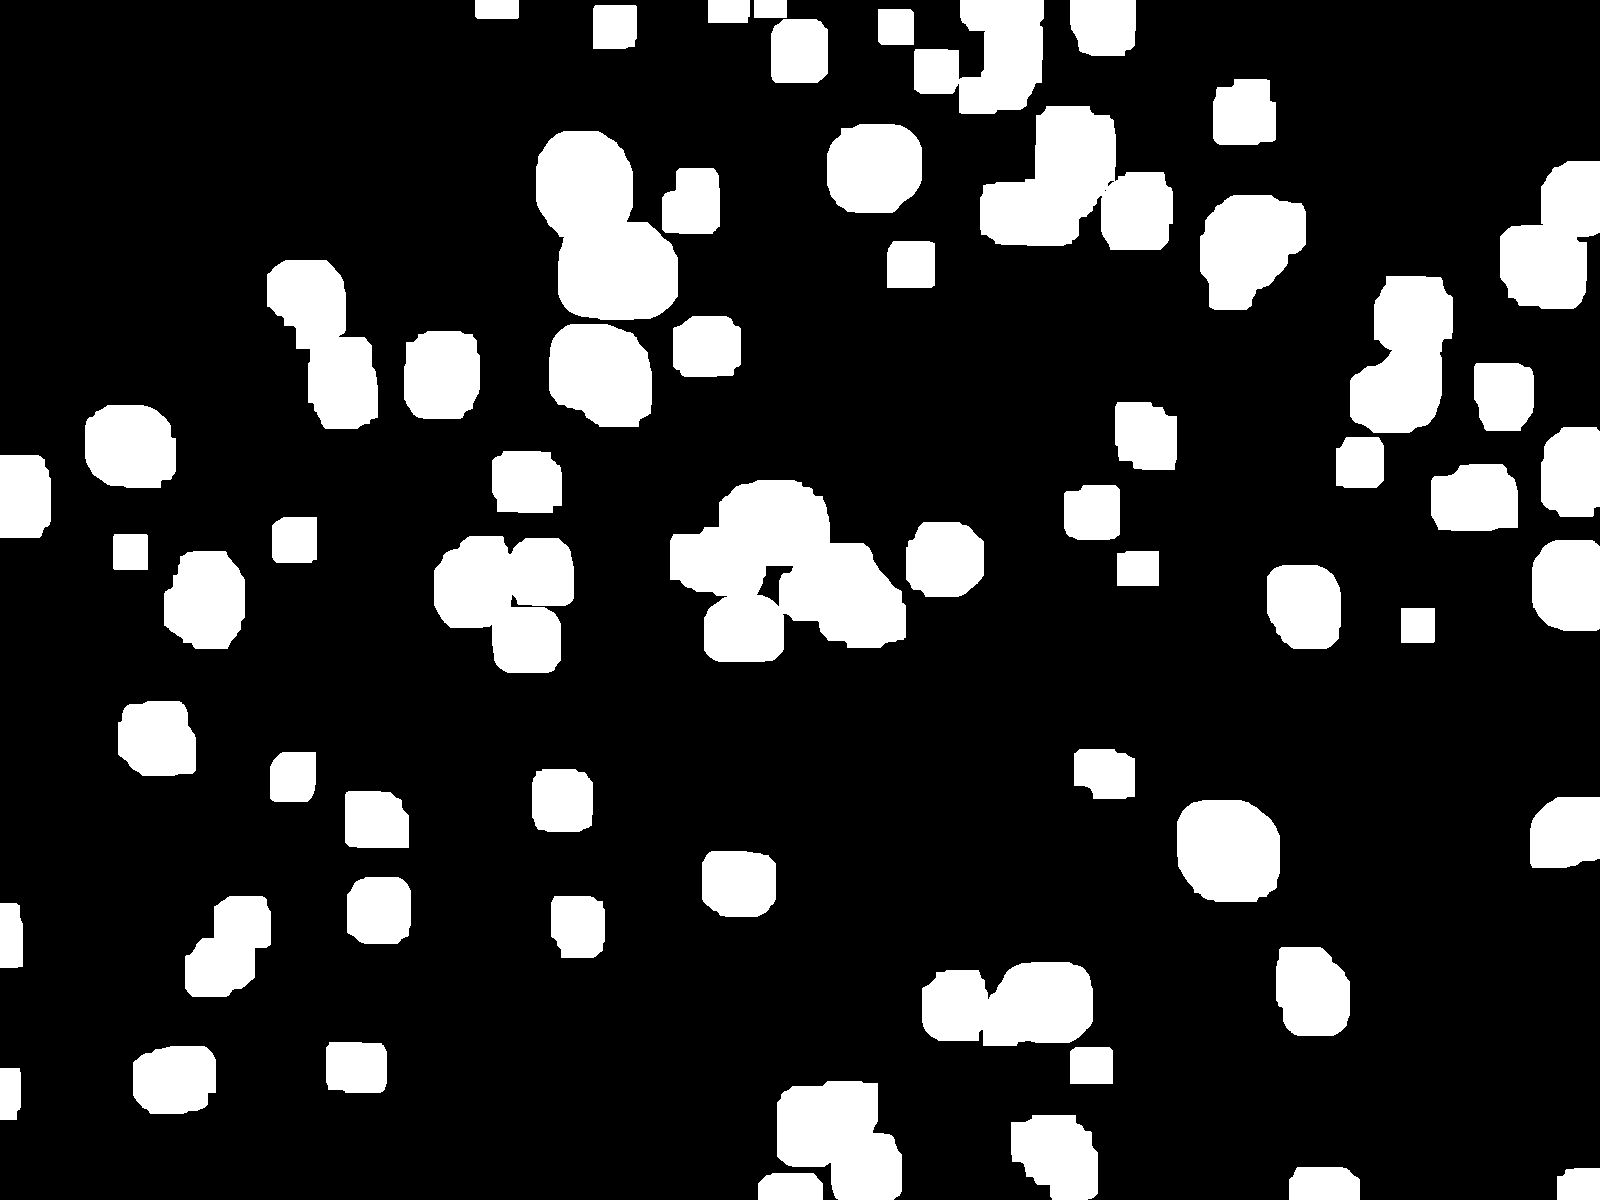
\includegraphics[width=0.95\linewidth]{Figures/Chapter2/3a.png}
	Розширене зображення за 2 ітерації
	\endminipage\hfill
	\minipage{0.5\textwidth}
	\centering	
	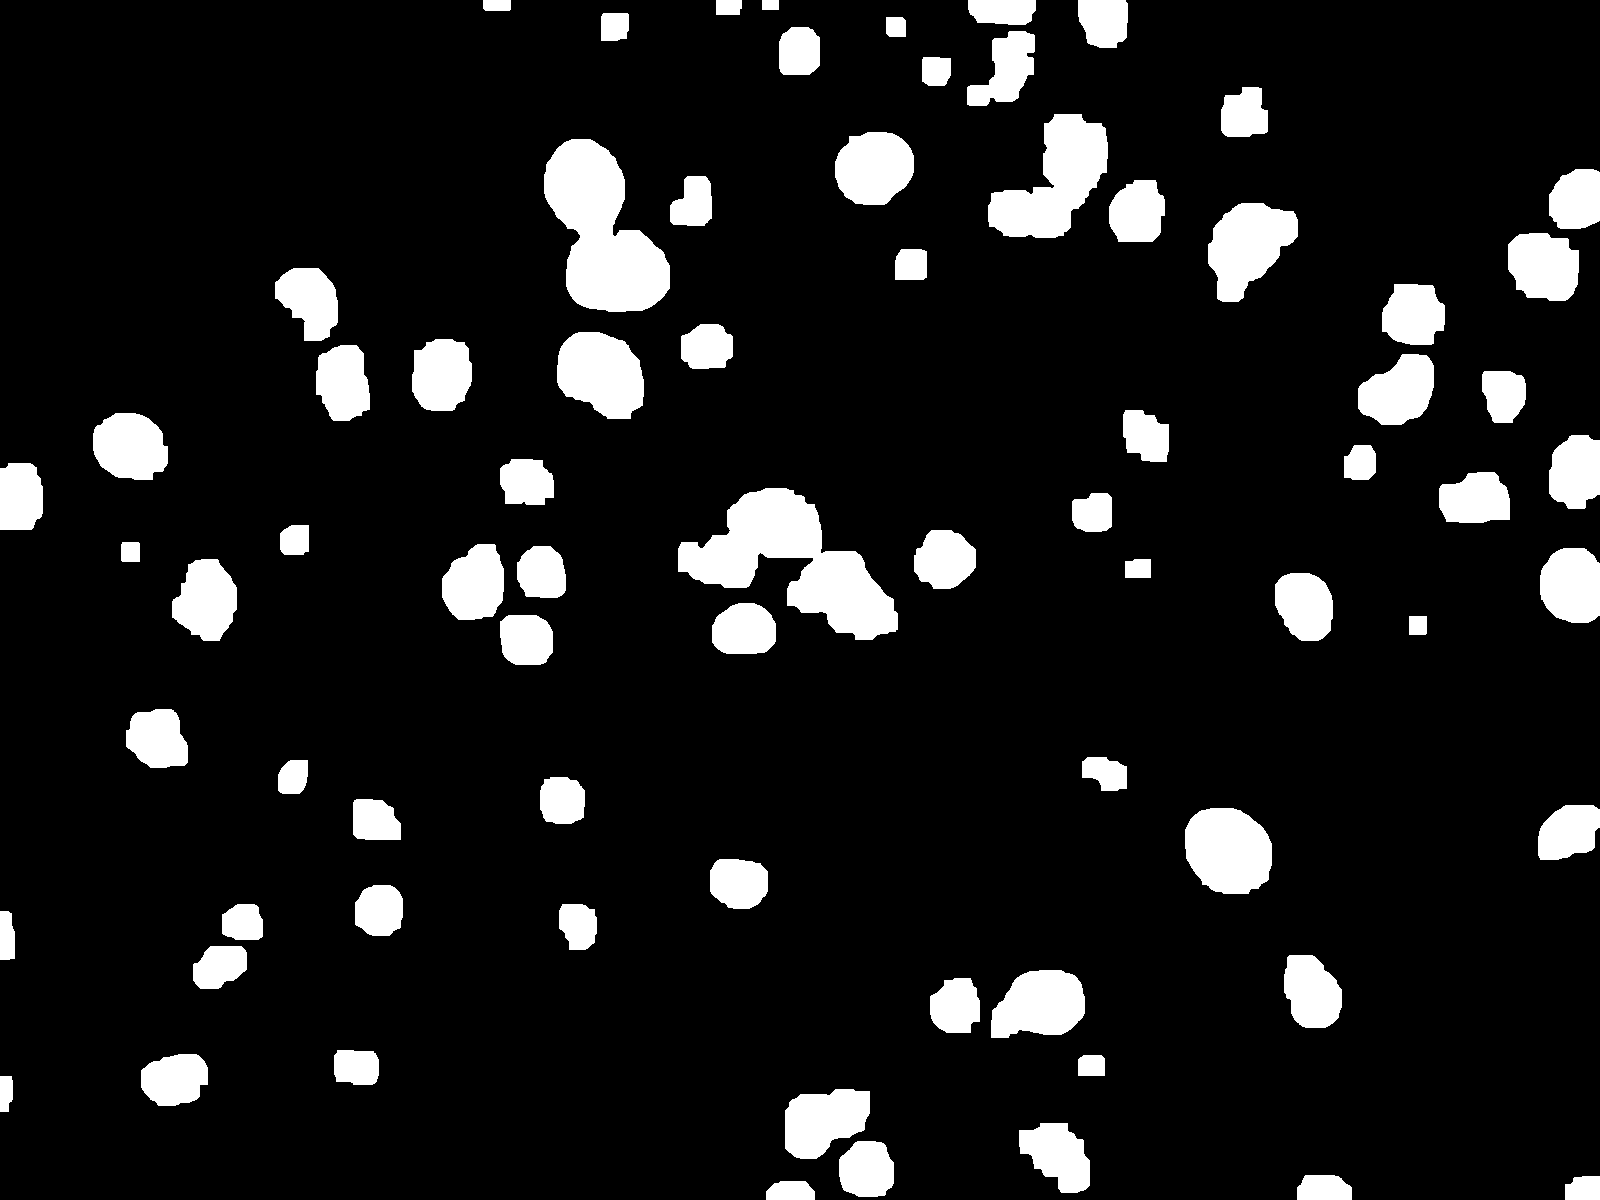
\includegraphics[width=0.95\linewidth]{Figures/Chapter2/3b.png}
	Відкриття зображення за 2 ітерації
	\endminipage\hfill
	
	\caption{Морфологічні операції над бінарним зображенням (Мал. \ref{fig:binarized_cells}).}
	\label{fig:morph_cells}
\end{figure}


\subsection{Трансформація дистанції}

\begin{figure}[t!]
	\minipage{0.5\textwidth}
	\centering	
	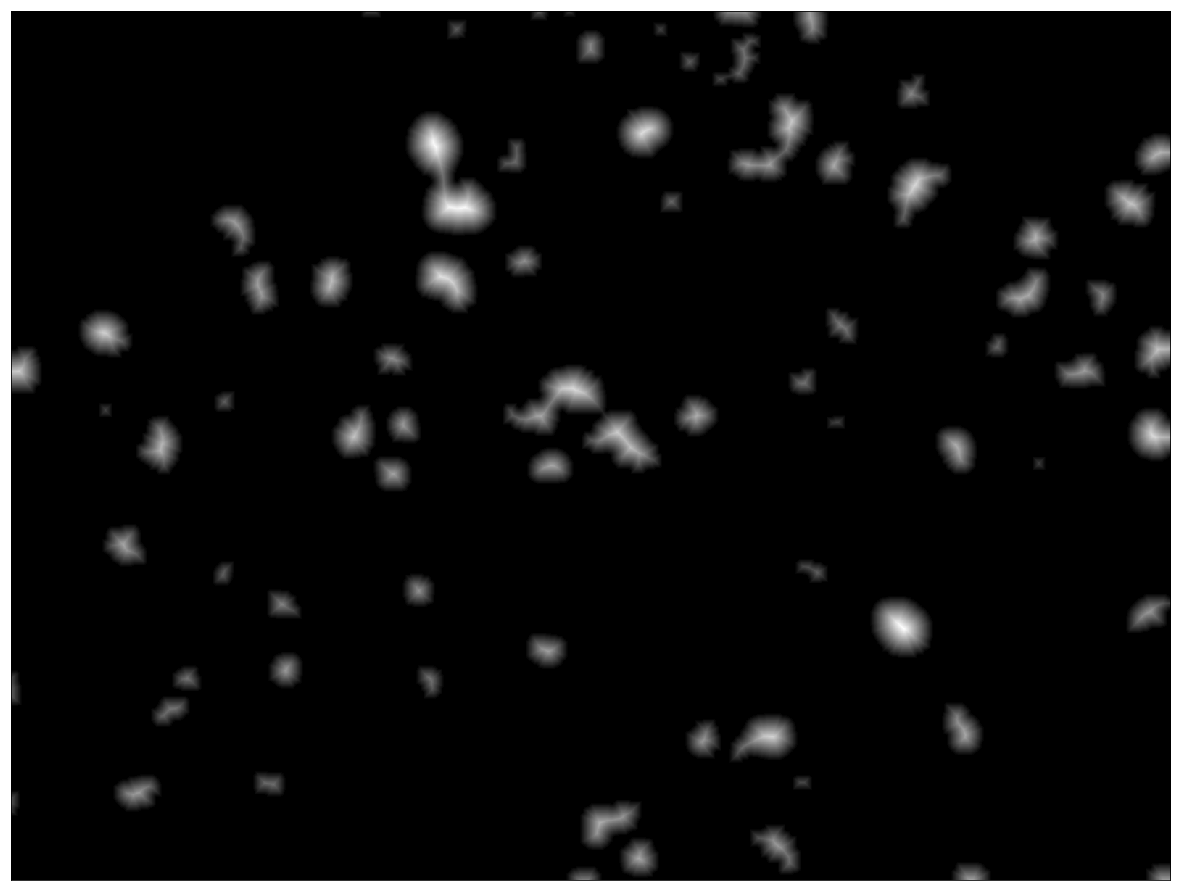
\includegraphics[width=0.95\linewidth]{Figures/Chapter2/4a.png}
	Трансформація дистанції
	\endminipage\hfill
	\minipage{0.5\textwidth}
	\centering	
	
\includegraphics[width=0.95\linewidth]{Figures/Chapter2/4b.png}
	\(sureFG\)
	\endminipage\hfill
	
	\caption{Трансформація дистанції.}
	\label{fig:dist_transform}
\end{figure}

Трансформація дистанції (Dіstance Transformatіon) є також операцією математичної мор- фології. Кожному пікселю переднього плану (що належить \(E\)) бінарного зображення \(E \subseteq \mathbb{Z}^d\) ставиться у відповідність відстань цієї точки до найближчого пікселя заднього плану (що не належить \(E\)). Для бінарних зображень найчастіше використовують Евклідову відстань, тобто для зображення \(E \subseteq F = \{1, 2, \dots, heіght\} \times \{1, 2, \dots, wіdth\}\), кожній точці \(z = (z_x, z_y) \in E\) ставимо у відповідність:
\begin{equation*}
DT(z) = \inf_{(x, y) \in F}{(|x - z_x| + |y - z_y|)}
\end{equation*}

Результат цієї операції для \(E = threshOpenіng\) можна інтерпретувати як показник вірогідності, що піксель \(z = (z_x, z_y)\) належить інтерфазному ядру клітини букального епітелію. Отже, можна задати емпіричне правило, за яким будемо приймати певні пікселі як \enquote{точно належать ядру клітини}:
\begin{equation}\label{eq:sure_fg}
DT(z) \geq \alpha \cdot \sup_{s \in E}{DT(s)} \Rightarrow \text{\enquote{z точно належать ядру клітини}}.
\end{equation}

Позначимо множину, що задовольняє цю нерівність, як \(sureFG\). Множник \(\alpha = 0.475\) був обраний експериментальним чином, на досліджуваних даних. Тут також використо- вується припущення, що усі ядра клітин мають приблизно однаковий розмір, а отже, центри цих клітин будуть знаходитись на приблизно однакому відстані від точок заднього плану. Для інших задач, дані яких зібрані за інших умов, слід обрати інший множник.

У (\ref{fig:dist_transform}) показано результат трансформації відстані та обчислення \(sureFG\) над бінарним зображенням \(threshOpenіng\), зображеним на (\ref{fig:morph_cells}). На \(sureFG\) ядра не дотикаються, завдяки обраному параметру \(\alpha\), тобто наш метод сегментації коректно обробляє ситуації, коли клітини торкаються чи частково перекриваються.

Використовуючи алгоритм що запропонований у \citep{bib:cooldisttrans} який використовує так звану рекур- сивну морфологію, можна обчислити трансформацію дистанції за два обходу. Для пов- ного виявлення окремих клітин, використаємо алгоритм водоподілу.

\subsection{Алгоритм водоподілу}

Трансформація водоподілу (Watershed) розглядає одноканальне зображення як топогра- фічну карту, де значення пікселя відображає висоту цієї точки. 

Починаючи з точок локальних мінімумів (або з заданих точок), кожна “яма” запов- нюється рідиною різних кольорів. З підвищенням рівня рідини, настає момент, коли дві рідини різного кольору починають змішуватися. Щоб уникнути цього, будуються границі між регіонами цих рідин. Границі будуються, доки рівень рідини не стане вищим за найвищу точку карти. Побудовані границі є результатами сегментації.

Використаємо цю ідею для сегментації ядер клітин. Кожну зв'язну компоненту \(sureFG\) пофарбуємо в певний \enquote{колір}. Назвемо таку сегментацію \enquote{набором маркерів}. Позначимо
\begin{equation*}
sureBG = E \setminus zoneOfInterest
\end{equation*}

Зв'язну множину пікселів заднього плану \(sureBG\) також пофарбуємо в якийсь колір. Непофарбованою залишається така множина:
\begin{equation*}
unknownRegion = zoneOfInterest \setminus sureFG
\end{equation*}

Тоді алгоритм водоподілу з заданими маркерами наступний \citep{bib:watershed}:

\begin{megaalgorithm}[H]
	\caption{Алгоритм водоподілу Майера з заданими маркерами}
	\SetKwInOut{Input}{Вхід}\SetKwInOut{Output}{Вихід}
	
	\Input{Зображення $X$ розміром $m \times n$, набір маркерів}
	\Output{Сегментація}
	\BlankLine 
	
	0. Будемо вважати, що \enquote{затоплення} починається саме с пікселів маркерів.\;
	1. Сусідні пікселі кожного маркеру додаємо в чергу з пріоритетом, де рівень пріоритету залежить від величини градієнту пікселя.\;
	2. Розглядається піксель з найменшим рівнем пріоритету. Якщо сусідні пікселі вже пофарбовані та мають однаковий колір, то фарбуємо цей піксель у колір сусідів. Усі сусіди, які ще не пофарбовані та ще не належать до черги з пріоритетом, додаються у чергу.\;
	3. Повторюємо крок 2, поки черга не стане пустою.\;
	4. Незафарбовані пікселі є границями водоподілу.\;
\end{megaalgorithm}

\begin{figure}[t!]
	\minipage{0.5\textwidth}
	\centering	
	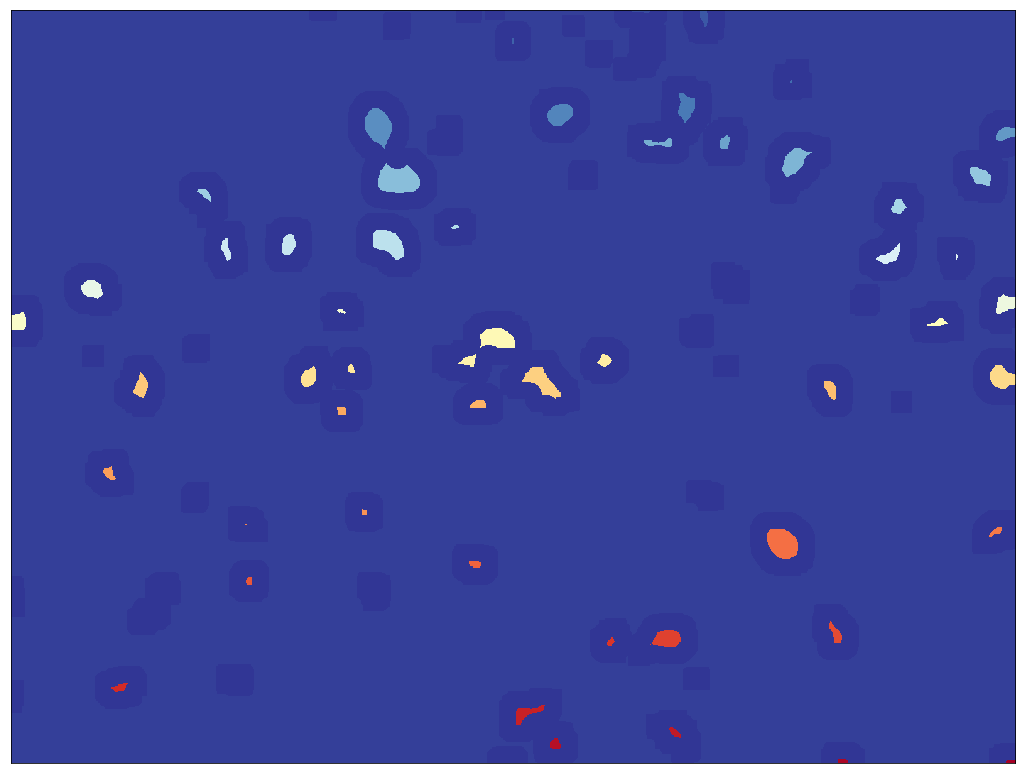
\includegraphics[width=0.95\linewidth]{Figures/Chapter2/5a.png}
	Маркери
	\endminipage\hfill
	\minipage{0.5\textwidth}
	\centering	
	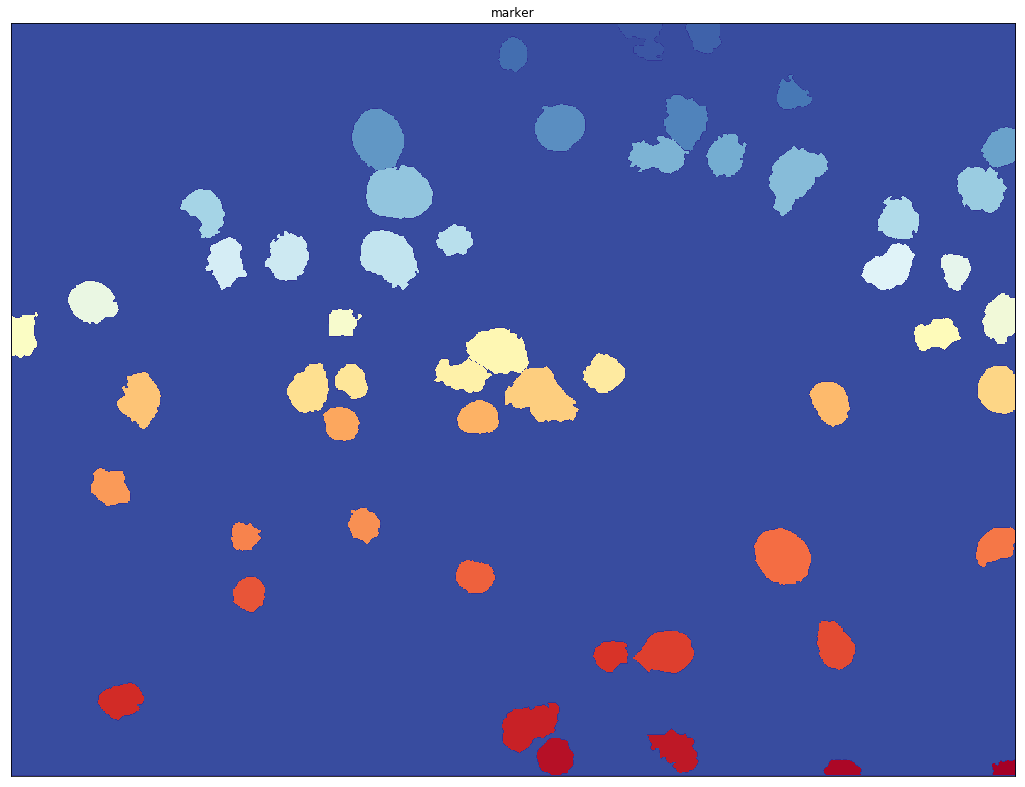
\includegraphics[width=0.95\linewidth]{Figures/Chapter2/5b.png}
	Кінцевий результат сегментації
	\endminipage\hfill
	
	\caption{Результат роботи алгоритму водоподілу (watershed).}
	\label{fig:watershed}
\end{figure}

\subsection{Кінцевий алгоритм сегментації}

Отже, кінцевий алгоритм сегментації інтерфазних ядер букального епітелію виглядає наступним чином:

\begin{megaalgorithm}[H]
	\caption{Сегментація ядер}
	\SetKwInOut{Input}{Вхід}\SetKwInOut{Output}{Вихід}
	
	\Input{Зображення $X$ розміром $m$}
	\Output{Зображення $Y$ такого ж розміру, де різні ядра зображені різними кольорами}
	\BlankLine 
	
	\(gray \leftarrow \text{сіре зображення X (grayscale)} \)\;
	\(blured \leftarrow \text{медіанна фільтрація }\, gray\, \text{ з вікном радіусом }\, r = 2\)\;
	\(thresh \leftarrow \text{бінаризація Оцу для }\, blured\)\;
	\(threshOpenіng \leftarrow\) морфологічне відкриття \(thresh\) з ядром \(9 \times 9\) за 2 ітерації\;
	\(zoneOfіnterest \leftarrow\) морфологічне розширення \(openіng\) з ядром \(9 \times 9\) за 2 ітерації\;
	\(dіstTransform \leftarrow\) трансформація відстані для \(threshOpenіng\)\;
	\(sureFG \leftarrow z\), які задовольняють формулу (\ref{eq:sure_fg})\;
	\(unknownRegіon \leftarrow zoneOfіnterest \setminus sureFG\)\;
	\(markers \leftarrow\) зв'язні компоненти \(sureFG \cup sureBG\)\;
	Виконати алгоритм водоподілу.
	
\end{megaalgorithm}

\begin{figure}[t!]
	\minipage{0.25\textwidth}
	\centering	
	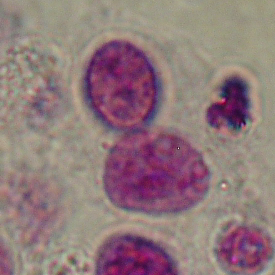
\includegraphics[width=0.97\linewidth]{Figures/Chapter2/6a1.png}
	
\includegraphics[width=0.97\linewidth]{Figures/Chapter2/6b1.png}
	
\includegraphics[width=0.97\linewidth]{Figures/Chapter2/6c1.png}
	\endminipage\hfill
	\minipage{0.25\textwidth}
	\centering	
	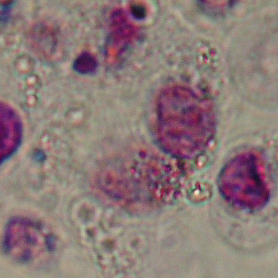
\includegraphics[width=0.97\linewidth]{Figures/Chapter2/6a2.png}	
	
\includegraphics[width=0.97\linewidth]{Figures/Chapter2/6b2.png}	
	
\includegraphics[width=0.97\linewidth]{Figures/Chapter2/6c2.png}
	\endminipage\hfill
	\minipage{0.25\textwidth}
	\centering	
	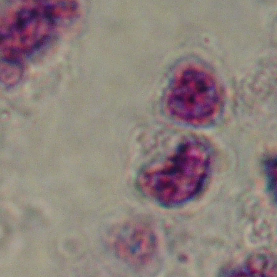
\includegraphics[width=0.97\linewidth]{Figures/Chapter2/6a3.png}	
	
\includegraphics[width=0.97\linewidth]{Figures/Chapter2/6b3.png}	
	
\includegraphics[width=0.97\linewidth]{Figures/Chapter2/6c3.png}
	\endminipage\hfill
	\minipage{0.25\textwidth}
	\centering	
	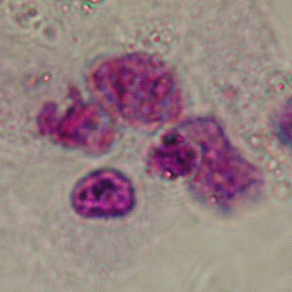
\includegraphics[width=0.97\linewidth]{Figures/Chapter2/6a4.png}	
	
\includegraphics[width=0.97\linewidth]{Figures/Chapter2/6b4.png}	
	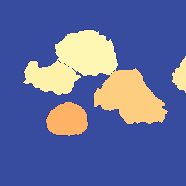
\includegraphics[width=0.97\linewidth]{Figures/Chapter2/6c4.png}
	\endminipage\hfill
	
	\caption{Випадки, коли ядра торкаються чи частково перекриваються.}
	\label{fig:amazing_segmentation}
\end{figure}

\bigskip
На (Мал. \ref{fig:amazing_segmentation}) бачимо, що наш алгоритм коректно сегментує також ті випадки, коли ядра клітин торкаються одне одного.

%----------------------------------------------------------------------------------------
%	SECTION 2

%----------------------------------------------------------------------------------------

\section{Нормалізація зображень}

Для нейронної мережі важливо переконатися, що вхідні дані нормалізовані. Для випадку зображень інтерфазних ядер букального епітелію, зображення можуть бути отримані у трохи різних умовах. Це може вплинути на швидкість тренування нейронної мережі, а також на точність розпізнавання.

Задньому плану зображення присвоюємо значення \(0\), щоб воно не активувало нейрони у мережі. Виконуємо нормалізацію гістограми для зображення одного ядра клітини так, щоб пікселі ядра приймали значення від \(0\) до \(255\). Це також може надати прискорення тренуванню нейронної мережі, оскільки більший діапазон значень означає більшу різ- ницю градієнтів у різних точках зображення.

Використовуючи попередні результати, видалимо задній план із зображення. Ядро клі- тини нормалізуємо за допомогою еквалізації гістограми, результат показано на  (Мал. \ref{fig:normalized_cells}).


\begin{figure}[t!]
	\minipage{0.2\textwidth}
	\centering
	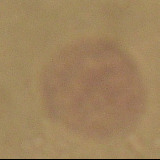
\includegraphics[width=0.95\linewidth]{Figures/Chapter2/7a1.png}	
	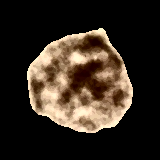
\includegraphics[width=0.95\linewidth]{Figures/Chapter2/7a2.png}	
	\endminipage\hfill
	\minipage{0.2\textwidth}
	\centering	
	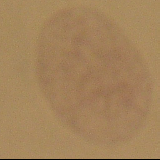
\includegraphics[width=0.95\linewidth]{Figures/Chapter2/7b1.png}
	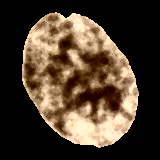
\includegraphics[width=0.95\linewidth]{Figures/Chapter2/7b2.png}
	\endminipage\hfill
	\minipage{0.2\textwidth}
	\centering	
	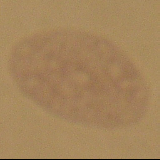
\includegraphics[width=0.95\linewidth]{Figures/Chapter2/7c1.png}
	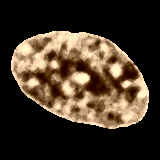
\includegraphics[width=0.95\linewidth]{Figures/Chapter2/7c2.png}
	\endminipage\hfill
	\minipage{0.2\textwidth}
	\centering	
	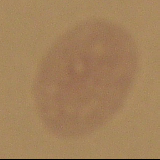
\includegraphics[width=0.95\linewidth]{Figures/Chapter2/7d1.png}
	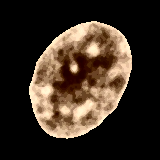
\includegraphics[width=0.95\linewidth]{Figures/Chapter2/7d2.png}
	\endminipage\hfill
	\minipage{0.2\textwidth}
	\centering	
	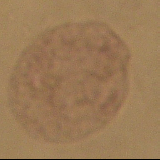
\includegraphics[width=0.95\linewidth]{Figures/Chapter2/7e1.png}
	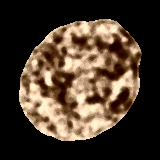
\includegraphics[width=0.95\linewidth]{Figures/Chapter2/7e2.png}
	\endminipage\hfill	
	
	\caption{Нормалізація зображень.}
	\label{fig:normalized_cells}
\end{figure}

%----------------------------------------------------------------------------------------
%	SECTION 4
%----------------------------------------------------------------------------------------

\section{Фільтр на основі еліпсоїдів Петуніна}

Згідно з роботою \parencite{bib:petuninfilter}, фільтр зображень на основі використання еліпсоїдів Петуніна має багато переваг над медіанним фільтром. У випадку фільтрації зображень інтерфазних ядер клітин, цей метод краще зберігає форму текстури. Отже, його можна використо- вувати для попередньої обробки даних для фрактального аналізу.

\subsection{Еліпсоїди Петуніна}

Нехай маємо множину точок \(M = \left\{x_1, x_2, \dots, x_n\right\}\), де \(x_i \in \mathbb{R}^m\) -- множина точок у \(m\)-вимірному просторі. Знайдемо точки \(x_l, x_k\) такі, щоб
\begin{equation*}
\sup_{x_i, x_j \in M}{\|x_i - x_j\|} = \|x_l - x_k\|
\end{equation*}
тобто відрізок \(L = x_l x_k\) -- діаметр множини точок \(M\). Повернемо і перенесемо систему координат так, щоб діаметр \(L\) належав \(O_{x'_1}\), де \(x'_1, x'_2, \dots, x'_n\) -- координати множини \(M\) у новій системі координат. 

Побудуємо найменший прямокутний паралелепіпед у \(\mathbb{R}^m\), який містив би елементи мно- жини \(M' = \left\{x'_1, x'_2, \dots, x'_n\right\}\). Стискаючи цей найменший прямокутний паралелепіпед, відобразимо його точки у гіперкуб. Знайдемо центр \(x_0\) гіперкуба та обчислимо відстані \(r_1, r_2, \dots, r_n\) від нього до кожної точки. 

Знайдемо найбільше \(R = \max{(r_1, r_2, \dots, r_n)}\) та побудуємо гіперкулю навколо центру \(x_0\) з радіусом \(R\). Зробимо обернене перетворення розтягу, повороту та переносу, отримаємо еліпсоїд Петуніна у \(m\)-вимірному просторі для множини \(M\). Система еліпсоїдів, отрима- них з кіл радіусами \(r_i\), де \(i \in 1, \dots n\) називається концентрованою системою еліпсоїдів Петуніна для множини \(M\).

Для системи концентрованих еліпсоїдів також справжується властивості, що є наслід- ками роботи Хілла \citep{bib:hill} та детально описані та доведені у \citep{bib:lyashko}.

\subsection{Фільтр зображень на основі еліпсоїдів Петуніна}

Нехай маємо на вході зображення, кожен піксель якого має \(d\) каналів. Зображення розглядається як відображення \(M: \mathbb{Z^2} \rightarrow \mathbb{R}^d\), тобто кожній координаті присвоюється \(d\)-канальне значення. Для кожного пікселя зображення, розглядаємо ще декілька пікселів, координати яких знаходяться в радіусі \(r\) від цього пікселя. Побудуємо для множини значень цих пікселів концентровану систему еліпсоїдів Петуніна, та у вихідному зобра- женні присвоїмо пікселю з тими ж координатами значення, яке відповідає внутрішньому (або центральному) еліпсоїду.

Детальний алгоритм виглядає наступним чином:

\begin{megaalgorithm}[H] \label{alg:petuninfilter0}
	\caption{Фільтр Петуніна}
	\SetKwInOut{Input}{Вхід}\SetKwInOut{Output}{Вихід}
	
	\Input{Зображення $X$ розміром $w \times h$, радіус ядра (вікна фільтру) \(r\)}
	\Output{Зображення $Y$ такого ж розміру}
	\BlankLine 
	
		
	\For{\(i = 1 \textup{ to } w \)}{
		\For{\(j = 1 \textup{ to } h \)}{
			\(D \leftarrow \text{нескінченний відрізок}\)\;
			\For {\(k = -r \textup{ to } r\)}{
			\For {\(l = -r \textup{ to } r\)}{
			\For {\(o = -r \textup{ to } r\)}{
			\For {\(p = -r \textup{ to } r\)}{
				Якщо \(\|D\| < \|X_{i+k, j+l} - X_{i+o, j+p}\|\) то \(D \leftarrow X_{i+k, j+l} X_{i+o, j+p}\) 
			}}}}
			Побудувати систему концентрованих еліпсоїдів Петуніна, маючи діаметр \(D\)\;
			$Y_{i,j} \leftarrow \textup{значення, що відповідає внутрішньому (або центральному) еліпсоїду}$\;
		}		
	}
\end{megaalgorithm}


\subsection{Швидкий алгоритм на основі динамічного програмування}

Незважаючи на переваги фільтру на основі еліпсоїдів Петуніна над медіанним фільтром (Алгоритм \ref{alg:petuninfilter0}) має серйозний недолік. Так, для зображення розміром \(w \times h\) та фільтру радіусом \(r\), асимптотична оцінка швидкості цього алгоритму становить:
\begin{equation*}
O\left( w \cdot h \cdot r^4 \right).
\end{equation*}

Для порівняння, асимптотична оцінка швидкості швидкого алгоритму медіанної фільтра- ції (Алгоритм \ref{alg:medianfilter}) або фільтра Гауса становить
\begin{equation*}
O\left(
\min\{w, h\} \cdot r^2 + w \cdot h \cdot r
\right).
\end{equation*}

Отже, при великих розмірах ядра (наприклад, \(r > 10\)) та великому об'ємі зображень, фільтр зображень на основі еліпсоїдів Петуніна значно повільніше працює, ніж інші алгоритми фільтрації. Основна причина -- повільний пошук діаметру. 

Існує багато швидких алгоритмів пошуку діаметру множини точок у \(d\)-вимірному прос- торі. Так, наприклад, Har-Peled запропонував евристичний алгоритм знаходження діа- метру \citep{bib:harpeled}. У \citep{bib:diamset} запропоновано детермінований алгоритм, що дозволяє знайти діаметр за час \(O\left( n \log n \right)\), де \(n\) -- кількість точок множини. Недоліком цих алгоритмів при викорис- танні для фільтру на основі еліпсоїдів Петуніна є те, що незважаючи на меншу асимпто- тику, ці алгоритми при невеликої кількості точок працюють не швидше, ніж простий алгоритм (повний перебір) пошуку діаметру. Оскільки розміри фільтрів більших ніж 21 майже не мають практичного використання, ми не можемо використовувати ці алгоритми для прискорення процесу пошуку діаметру.

Можна помітити, що при \enquote{пересування} вікна фільтру, ми повторно виконуємо деякі обчислення. Якщо зможемо оптимальніше виконувати обчислення (без повторень), то зможемо швидше фільтрувати зображення. Автором цієї роботи пропонується алгоритм на основі динамічного програмування, що значно прискорює процес пошуку діаметру.

Опишемо структуру даних \enquote{двовимірна черга що зберігає діаметр}. Ця структура пред- ставляє собою двійка \(\left(H, p\right)\), де p -- координата центру вікна фільтру відносно зображення \(X\), а H -- таблиця розміром \((2r + 1) \times (2r + 1)\), кожен елемент якого зберігає діаметр множини точок, що відповідає пікселям, що потра- пляють у фільтр нижче чи правіше, тобто:
\begin{equation}
\label{eq:queueinit}
H_{i, j} = \left\| D(\{ X_{y, x} \big| x \in [(p_x + i), (p_x + r)]_{\mathbb{Z}}, y \in [(p_y + j), (p_y + r)]_\mathbb{Z} \}) \right\|,\,\, i, j \in -r \dots r
\end{equation}

\par
де \(D\) -- діаметр множини, \(X_{y, x}\) -- \(d\)-вимірне значення пікселю з координатами \((y, x)\). Очевидно, що в \(H_{-r, -r}\) зберігається діаметр множини точок значень пікселів, що потра- пляють у вікно фільтру. 

\par
Опишемо алгоритм оновлення таблиці \(H\) при пересуванні фільтру праворуч. Алгоритм при пересуванні фільтру вниз задається аналогічним чином.

\bigskip

\begin{megaalgorithm}[H] \label{alg:2dqueuetranslation}
	\caption{Оновлення таблиці \(H\) при пересуванні вікна фільтру праворуч}	
	\SetKwInOut{Input}{Вхід}\SetKwInOut{Output}{Вихід}
	
	\Input{Зображення $X$, радіус ядра (вікна фільтру) \(r\), двовимірна черга що зберігає діаметр \((H, p)\) що відповідає вікну}
	\Output{двовимірна черга що зберігає діаметр \((H', p')\) що відповідає вікну після зміщення праворуч на 1 піксель}
	\BlankLine 
	
	\(H'_{r, r} \leftarrow 0\)\;
	\For{\(i = r - 1 \textup{ downto } -r\)}{
		\(H'_{r, j} \leftarrow \max\left\{ \max\left\{ \|X_{p_y+i, p_x+r} - X_{p_y+k, p_x+r}\| \quad \forall k \in i \dots r \right\}, \quad H'_{i+1, r} \right\}\)
	}
	\For{\(j = r - 1 \textup{ downto } -r\)}{
		\For{\(i = r \textup{ downto } -r\)}{
			\(H'_{i,j} \leftarrow \max\left\{ \max\left\{ \|X_{p_y+i,p_x+j} - X_{p_y+k, p_x+r}\| \quad \forall k \in i \dots r \right\}, \quad H'_{i+1, j}, \quad H'_{i, j+1} \right\}\)
		}
	}
\end{megaalgorithm}

Також опишемо алгоритм для обчислення \((H, p)\), знаючи \((H^{left}, p^{left})\) та \((H^{top}, p^{top})\), де \(p^{left} = (p_y, p_x-1)\), \(p^{top} = (p_y-1, p_x)\), тобто знаючи черги, що відповідають вікнам на піксель вище чи лівіше.

\begin{megaalgorithm}[H] \label{alg:2dqueueinstantiation}
	\caption{Обчислення таблиці \(H\) знаючи відповідні таблиці ліворуч та вище}	
	\SetKwInOut{Input}{Вхід}\SetKwInOut{Output}{Вихід}
	
	\Input{Зображення \(X\), радіус ядра (вікна фільтру) \(r\), двовимірні черги що зберігає діаметр \((H^{left}, p^{left})\) та \((H^{top}, p^{top})\) що відповідає вікну лівіше та вище відповідно}
	\Output{двовимірна черга що зберігає діаметр \((H, p)\)}
	\BlankLine 
	
	\(H_{r, r} \leftarrow 0\)\;
	\For{\(i = r \textup{ downto } -r\)}{
	\For{\(j = r \textup{ downto } -r\)}{
		\(H_{i,j} = \max\left\{
		H^{left}_{i, j+1}, \quad
		H^{top}_{i+1, j}, \quad
		H_{i, j+1}, \quad
		H_{i+1, j}, \quad
		\|X_{p_y+r, p_x+r} - X_{p_y+i, p_x+j}\|,
		\right\}\)
	}
	}
\end{megaalgorithm}

\par
Слід зазначити, що в (Алгоритм \ref{alg:2dqueuetranslation}) та (Алгоритм \ref{alg:2dqueueinstantiation}), після кожного кроку присвоєння значення діаметру, слід також у таблиці \(D_{i, j}\) зберігати точки кінців діаметру. Опишемо кінцевий алгоритм швидкої фільтрації зображення на основі системи концентрованих еліпсоїдів Петуніна:

\begin{megaalgorithm}[H] \label{alg:petuninfilter1}
	\caption{Швидкий алгоритм фільтрації Петуніна}
	\SetKwInOut{Input}{Вхід}\SetKwInOut{Output}{Вихід}
	
	\Input{Зображення \(X\) розміром \(w \times h\), радіус ядра (вікна фільтру) \(r\)}
	\Output{Зображення \(Y\) такого ж розміру}
	\BlankLine 
	
	Обчислити \((H_0, p_0 = (1, 1))\) згідно за формулою (\ref{eq:queueinit}), а також відповідний відрізок \(L_0\)\;
	\For{\(i = 1 \textup{ to } h \)}{
		За (Алгоритм \ref{alg:2dqueuetranslation}) обчислити \((H^{i, 1}, p^{i, 1} = (i, 1))\) та відповідний відрізок \(L^{i, 1}\)\;
		Побудувати систему концентрованих еліпсоїдів Петуніна, маючи діаметр \(L^{i,1}\)\;
		$Y_{i,1} \leftarrow \textup{значення, що відповідає внутрішньому (або центральному) еліпсоїду}$\;
	}
	\For{\(j = 1 \textup{ to } w \)}{
		За (Алгоритм \ref{alg:2dqueuetranslation}) обчислити \((H^{1, j}, p^{1, j} = (1, j))\) та відповідний відрізок \(L^{1, j}\)\;
		Побудувати систему концентрованих еліпсоїдів Петуніна, маючи діаметр \(L^{1,j}\)\;
		$Y_{1,j} \leftarrow \textup{значення, що відповідає внутрішньому (або центральному) еліпсоїду}$\;
	}

	\For{\(i = 1 \textup{ to } h \)}{
		\For{\(j = 1 \textup{ to } w \)}{
			За (Алгоритм \ref{alg:2dqueueinstantiation}) обчислити \((H^{i, j}, p^{i, j})\) та відповідний відрізок \(L^{i,j}\)\;
			Побудувати систему концентрованих еліпсоїдів Петуніна, маючи діаметр \(L^{i,j}\)\;
			$Y_{i,j} \leftarrow \textup{значення, що відповідає внутрішньому (або центральному) еліпсоїду}$\;
		}		
	}
\end{megaalgorithm}

\par
Очевидно, що (Алгоритм \ref{alg:2dqueuetranslation}) має асимптотичну оцінку \(O\left( r^3 \right)\), а (Алгоритм \ref{alg:2dqueueinstantiation}) має оцінку \(O\left(r^2\right)\). Тоді асимптотична оцінка для (Алгоритм \ref{alg:petuninfilter1}) дорівнює:
\begin{equation*}
O\left(
r^4 + r^3 \left(w + h\right) + w \cdot h \cdot r^2
\right)
\end{equation*}

Оскільки значення \(r\) значно менша ніж розмір зображення \(w \times h\), то (Алгоритм \ref{alg:petuninfilter1}) можна оцінити як
\begin{equation*}
O\left(w \cdot h \cdot r^2\right)
\end{equation*}

Що дорівнює швидкості звичайного алгоритму медіанної фільтрації.